\documentclass{article}
\usepackage[utf8]{inputenc}
\usepackage{graphicx}
\usepackage{amsmath, amsthm, amssymb}
\usepackage{multicol}
\usepackage{svg}
\usepackage{caption}
\usepackage{vmargin}
\usepackage[hidelinks]{hyperref}

\theoremstyle{definition}
\newtheorem{defi}{Definition}[section]
\newtheorem{theorem}{Theorem}[section]
\newtheorem{proposition}{Proposition}[section]
\newtheorem{lemma}{Lemma}[section]

\title{An investigation on $\mathbb{Z}/n\mathbb{Z}$}
\author{Xiaozhe Yao\footnote{https://yaonotes.org/lecture-notes.html}}
\date{28 Oct 2019}
\begin{document}

\maketitle
\begin{center}
    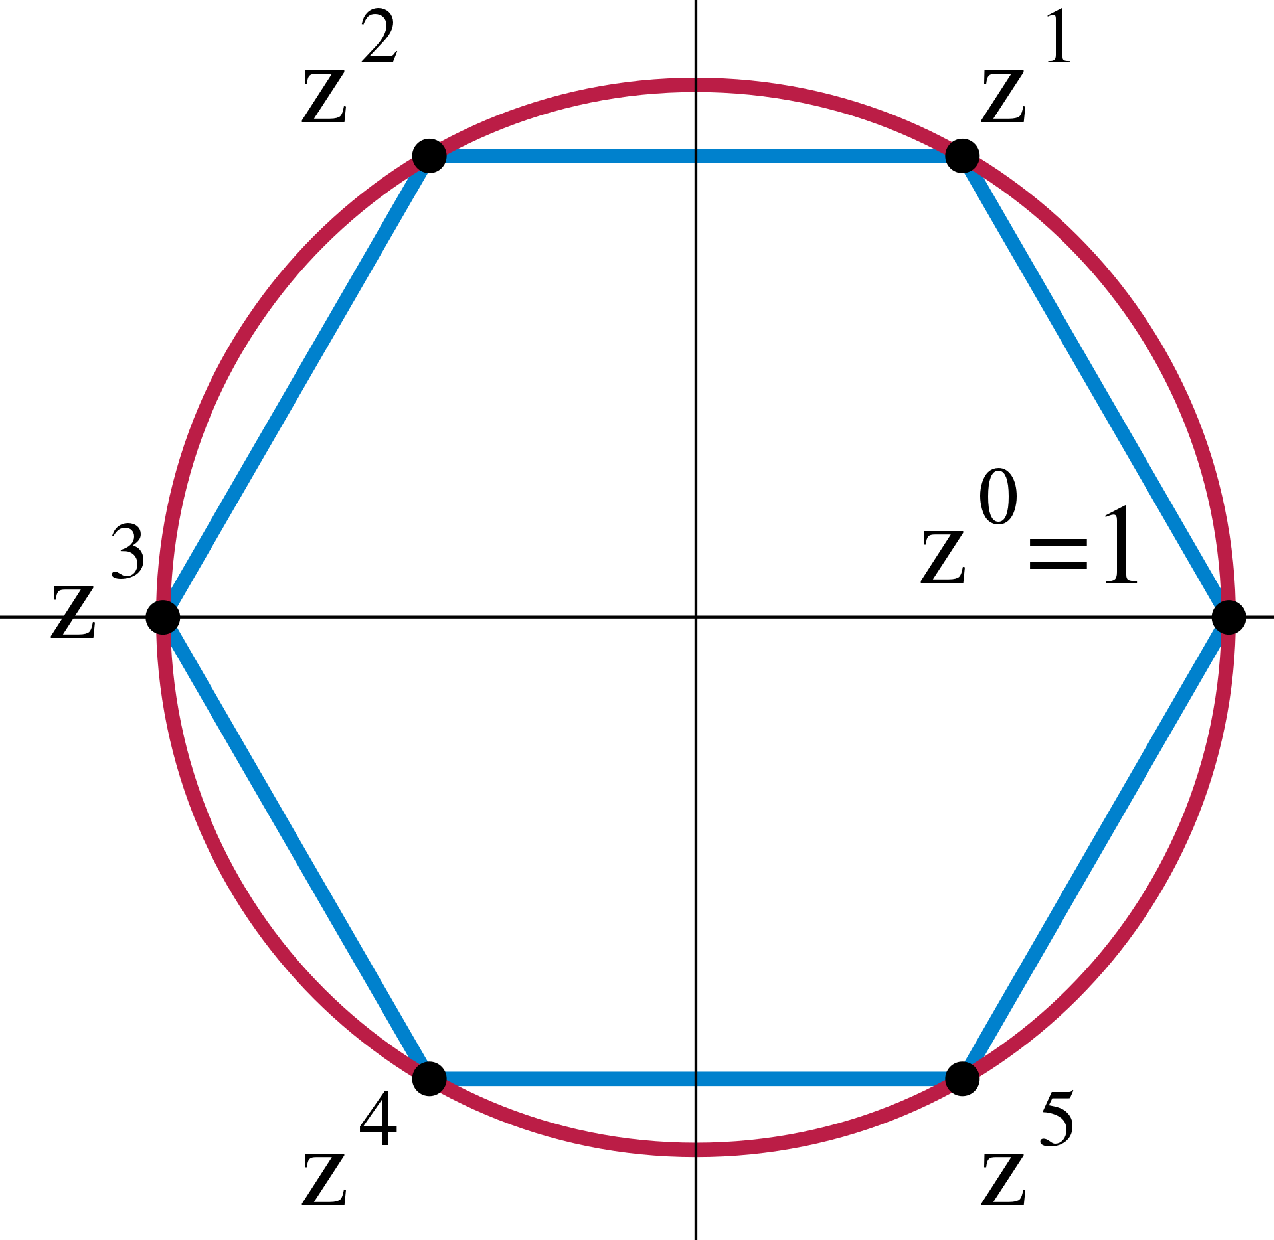
\includegraphics[width=60px]{Algebra/images/cyclic_group.pdf}
\end{center}
\section{Introduction}
$\mathbb{Z}/n\mathbb{Z}$ is the set of all congruence classes of the integers for a modulus $n$. It can be written as $\mathbb{Z}_n$, $\mathbb{Z}/n$ or $\mathbb{Z}/n\mathbb{Z}$. 

\section{Properties of $\mathbb{Z}$}

\subsection{Group, Ring and Field}

\begin{proposition}
$(\mathbb{Z},+)$ is a cyclic group
\end{proposition}

it can be generated by a fixed number of elements. For example, it can be generated by $1$, since $\forall x \in \mathbb{Z}, x = x \cdot 1$. It can be written as $\mathbb{Z}=\langle1\rangle$. Similarly we can get $\mathbb{Z}=\langle-1\rangle$. 

\begin{proposition}
In fact, $(\mathbb{Z},+)$ is the only infinite cyclic group, in the sense that every inifinite cyclic group is isomorphic to $(\mathbb{Z},+)$.
\end{proposition}

\textit{Proof:} Let $G=\langle a \rangle = \{a^k: k \in \mathbb{Z}\}$, we define $\phi = \mathbb{Z} \to G: \phi(k)=a^k$. The operation on $G$ is denoted as $\cdot$

We now prove $\phi$ is a isomorphism:

1) It is a homomorphism. \textit{Proof:} Let $k,l \in \mathbb{Z}$, then $\phi(k+l)=a^{k+l}=a^ka^l = \phi(k) \cdot \phi(l)$.

2) It is surjective. \textit{Proof:} As $G$ is cyclic, $\forall x\in G, \exists k \in \mathbb{Z} : x=a^k$. By the definiction of $\phi$, $\phi(k) = a^k = x$. i.e for any element $x$ in $G$, there is a $k$ such that $\phi(k)=x$. It is surjective.

3) It is injective. \textit{Proof:} $\forall m,n \in \mathbb{Z}, m \neq n \Rightarrow a^m \neq a^n$, $a^m=a^n \Rightarrow m=n$. $\hfill\blacksquare$

\begin{proposition}
$(\mathbb{Z},+,\cdot)$ is a ring.
\end{proposition}

\textit{Proof:} 1) $(\mathbb{Z},+)$ is an abelian group, the neutral is 0.

2) $\cdot$ is associative, the neutral element is 1.

3) $\cdot$ is distributive, regarding the addition. i.e. $a\cdot(b+c) = a\cdot b +a\cdot c$

4) $\cdot$ is commutative. $\hfill\blacksquare$

\begin{proposition}
$(\mathbb{Z},+,\cdot)$ is \textbf{not} a field.
\end{proposition}
Not every element in $\mathbb{Z}$ has an inverse, which is equivalent to $\mathbb{Z}$ is not closed under division. For example, $2x=1$, then $x\notin \mathbb{Z}$. It also indicates that $(\mathbb{Z}, \cdot)$ is not a group.

\subsection{Order}

$\mathbb{Z}$ is a totally ordered set without upper or lower bound. The order of integers is compatible with the algebraic operations in the following way:

1) If $a<b$ and $c<d$, then $a+c<b+d$.

2) If $a<b$ and $c>0$, then $ac<bc$.

It follows that $\mathbb{Z}$ is an ordered ring.

\subsection{Subgroup}

\begin{theorem}
Every non-trivial subgroup of $(\mathbb{Z},+)$ has the form $n\mathbb{Z}$.
\end{theorem}


\textbf{Lemma}
$n\mathbb{Z}$ is the subgroup of $\mathbb{Z}$. The proof is straightforward by definition.

\textit{Proof:} 

1) $n\mathbb{Z}$ is closed under addition. Let $x,y \in n\mathbb{Z}$, $x=n\cdot a, y=n\cdot b$, then $x+y = n\cdot a + n\cdot b=n\cdot(a+b) \in n\mathbb{Z}$
    
2) $n\mathbb{Z}$ is a group. The neutral element is $0 n\mathbb{Z}$, and every element has an inverse (Let $x=n\cdot a$, then $a\in \mathbb{Z}$, then $-a \in \mathbb{Z}$. Hence $n\cdot(-a) \in \mathbb{Z}$). In addition $+$ is associative. $\hfill\blacksquare$

\textbf{Proposition}
Every subgroup of $(\mathbb{Z}, +)$ has the form $n\mathbb{Z}$.


\textit{Proof:} Let H $\subseteq \mathbb{Z}$, we want to prove $H=n\mathbb{Z}, n \in \mathbb{Z}$.

1) For the trivial subset, $H=(\{0\}, +)$, $H=0\cdot \mathbb{Z}$.

2) If $H$ is non-trivial, let $n$ be the smallest positive element of $H$. If $n=1$, then $H=\mathbb{Z}$.

If $n\neq1$, Let $h\in H$ then $h=nq+r, q,r \in \mathbb{Z}, 0\leq r<n$. Then we have $r=h-nq \in \mathbb{H}$. Since $n$ is the smallest positive element of $H$, $r$ must be $0$. Hence we have $\forall h \in H$, $h=nq \in n\mathbb{Z}$. Thus $H=n\mathbb{Z}$. $\hfill\blacksquare$

\begin{proposition}
$\forall m,n \in \mathbb{Z}, \exists d\in \mathbb{Z}: m\mathbb{Z} + n\mathbb{Z}=d\mathbb{Z}$, where $d=gcd(m,n)$.
\end{proposition}

\textit{Proof:} Let $I=m\mathbb{Z}, J=n\mathbb{Z}$, we want to prove $I+J = gcd(m,n)\mathbb{Z}$. We can prove that $I+J \subseteq gcd(m,n)\mathbb{Z}$ and $gcd(m,n)\mathbb{Z}\subseteq I+J$.

1) Since $gcd(m,n)|n$, any multiple of $n$ is also multiple of $gcd(m,n)$, thus $I \subseteq gcd(m,n)\mathbb{Z}$. Similarly, $J \subseteq gcd(m,n)\mathbb{Z}$. Since $gcd(m,n)\mathbb{Z}$ is closed under addition, $I+J \subseteq gcd(m,n)$.

2) $gcd(m,n) = an+bm$. $an \in I$ and $bm \in J$. Therefore $gcd(m,n) \in I+J$. Since $I+J$ is closed under multiplication by any integer, we have $gcd(m,n)\mathbb{Z} \subseteq I+J$ 


\section{Properties of $\mathbb{Z}/n\mathbb{Z}$}

$\mathbb{Z}/n\mathbb{Z}$ is \textbf{not} a subgroup of $\mathbb{Z}$, it is not even a subset of $\mathbb{Z}$. The elements of $\mathbb{Z}/n\mathbb{Z}$ are equivalence classes of integers, not integers themselves. We usually write it as $\mathbb{Z}/n\mathbb{Z}=\{0,1,2,...n-1\} \subseteq \mathbb{Z}$ for simplification (but it is \textbf{not} technically correct!). But the group operation in $\mathbb{Z}/n\mathbb{Z}$ would have to be different than the operation in $\mathbb{Z}$. The operation on $\mathbb{Z}/n\mathbb{Z}$ is the addition over modular.

\subsection{Subgroups}

\begin{theorem}
All subgroups of $\mathbb{Z}/n\mathbb{Z}$ has the form $\mathbb{Z}/q\mathbb{Z}$, where $q|n$.

\textit{Proof:} Define the project $\phi: \mathbb{Z} \to \mathbb{Z}/n\mathbb{Z}$. Let $H$ be the subgroup of $\mathbb{Z}/n\mathbb{Z}$. Then we know $\phi^{-1}=q\mathbb{Z}$ is a subgroup of $\mathbb{Z}$.

\textbf{Lemma} The subgroups of cyclic group are still cyclic, and the order of a cyclic subgroup divides the order of the group. 

1) If $\phi^{-1}(H)=q\mathbb{Z}$, then $q|n$. Since $\mathbb{Z}/n\mathbb{Z}$ is cyclic, $H$ is cyclic too and the order of $H$ divides $n$. Now $\phi^{-1}(H)$ is a subgroup of $\mathbb{Z}$, and $0\in H$(Because $H$ is a group, so the neutral element must be in it). It follows that $n\mathbb{Z} \subseteq \phi^{-1}(H)$. As proved in \textbf{Theorem 2.1}, all subgroups of $\mathbb{Z}$ has the form $m\mathbb{Z}$, we know that $\phi^{-1}(H)$ has the form $q\mathbb{Z}$. In all, $n\mathbb{Z} \subseteq q \mathbb{Z}$. Which means $n = pq$ and thus $q|n$.

2) It is clear that $\phi(d\mathbb{Z}) = d\mathbb{Z}/n\mathbb{Z}$ and $\phi^{-1}(d\mathbb{Z}/n\mathbb{Z}) = d\mathbb{Z}$. If $m$ is any integer, then $\phi(m\mathbb{Z})=a\mathbb{Z}/n\mathbb{Z}$ where $a=gcd(m,n)$ and $\phi^{-1}(\phi(m\mathbb{Z}))=a\mathbb{Z}$. Thus we have $\phi^{-1}(\phi(m\mathbb{Z}))=m\mathbb{Z}$ only if $gcd(m,n)=m$, i.e. only if $m$ divides $n$. This is equivalent to the condition that $m\mathbb{Z}$ contains $n\mathbb{Z}$, the kernel of $\phi$. 

\end{theorem}

\end{document}